\documentclass[a4paper]{article}

%% Language and font encodings
\usepackage[english]{babel}
\usepackage[utf8x]{inputenc}
\usepackage[T1]{fontenc}

%% Sets page size and margins
\usepackage[a4paper,top=3cm,bottom=2cm,left=3cm,right=3cm,marginparwidth=1.75cm]{geometry}

%% Useful packages
\usepackage{amsmath}
\usepackage{pgfplots}
\pgfplotsset{compat=1.14}
\usepackage{graphicx}
\usepackage[colorinlistoftodos]{todonotes}
\usepackage[colorlinks=true, allcolors=blue]{hyperref}
\usepackage{subfig}
\usepackage{float}
\usepackage{multicol}

\title{The Dartboard Challenge}
\author{Joshua Van Leeuwen \& Karim Allaouat}

\begin{document}
\maketitle

\setcounter{section}{-1}
\section{Introduction}

This task introduces the ability to detect and locate instances of an object
class in images. This is important as this ability is used in many computer
vision applications. The task explores the Viola-Jones object detection
framework (an “off the shelf” face detector) and combines it with other
detection techniques to improve it. The image set used is from the popular
sport, darts.

\section{The Viola-Jones Object Detector}

The Viola-Jones object detection framework is the first object detection
framework to provide competitive object detection rates in real time. The
algorithm was used with a strong classifier trained using AdaBoost for
detecting human faces from the front.

\subsection*{Using the Detector on Human Faces}

\begin{figure}[H]
  \centering
  \subfloat[dart4.jpg.]{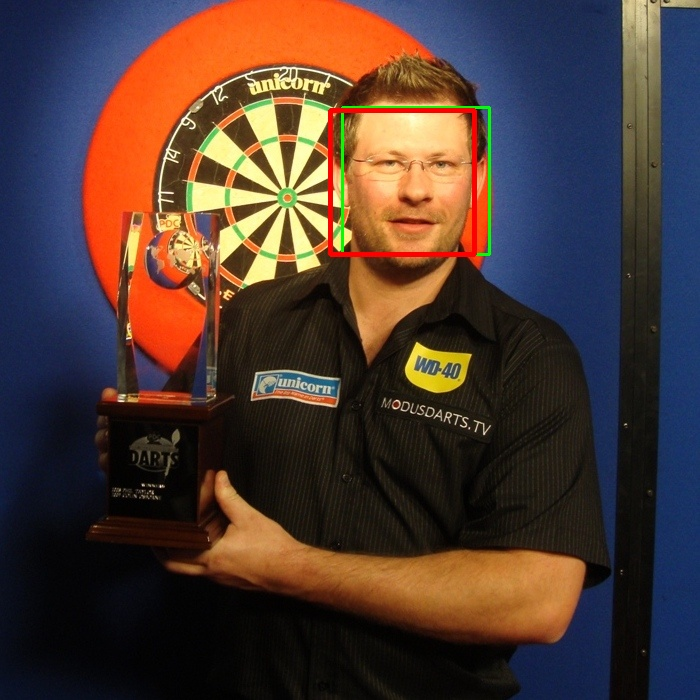
\includegraphics[width=\textwidth, height=20mm, keepaspectratio]{task1/out4.jpg}\label{fig:dart4}}
  \hfill
  \subfloat[dart5.jpg]{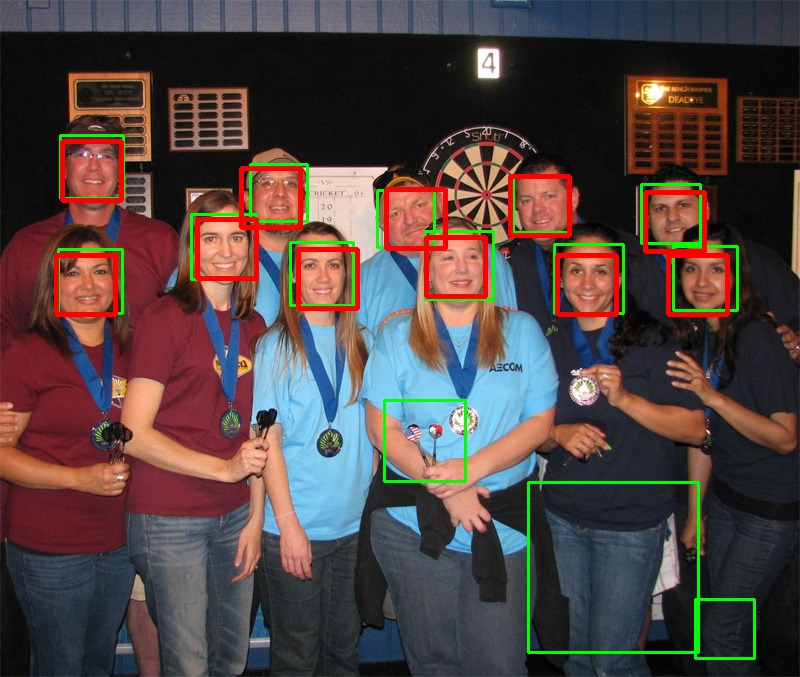
\includegraphics[width=\textwidth, height=20mm, keepaspectratio]{task1/out5.jpg}\label{fig:dart5}}
   \hfill
  \subfloat[dart13.jpg]{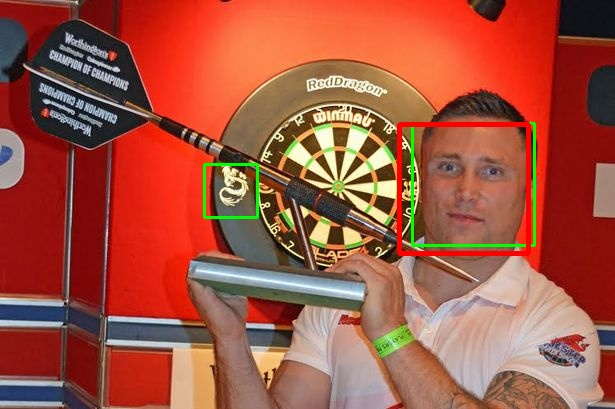
\includegraphics[width=\textwidth, height=20mm, keepaspectratio]{task1/out13.jpg}\label{fig:dart13}}
   \hfill
  \subfloat[dart14.jpg]{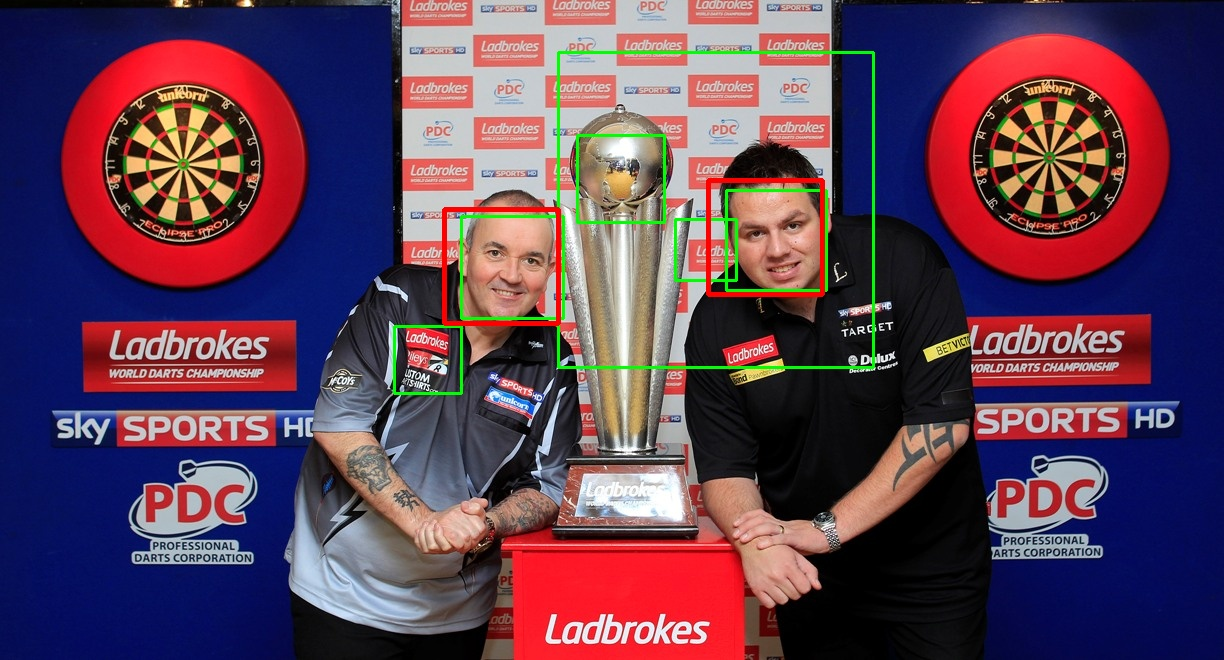
\includegraphics[width=\textwidth, height=20mm, keepaspectratio]{task1/out14.jpg}\label{fig:dart14}}
   \hfill
  \subfloat[dart15.jpg]{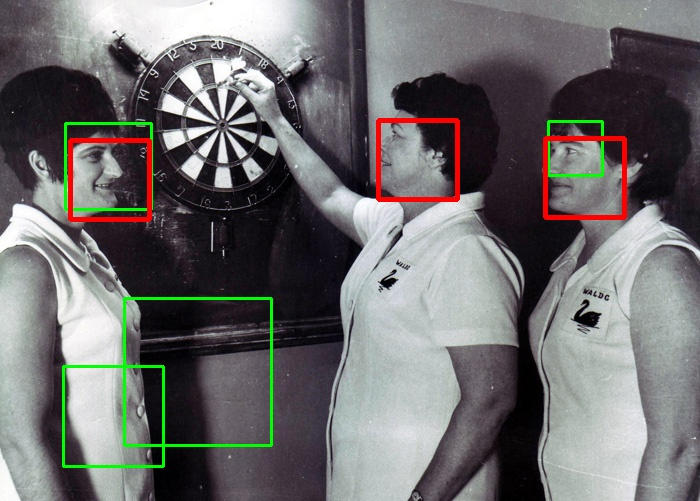
\includegraphics[width=\textwidth, height=20mm, keepaspectratio]{task1/out15.jpg}\label{fig:dart15}}
   \hfill
   \caption{Result of Viola-Jones Algorithm on Human Faces.}
\end{figure}

\subsection*{Assessing How the Detector Performs}

The TPR or True Positive Rate measures the proportion of relevant items that
are correctly identified. In this case it is the fraction of successfully
detected faces out of all valid faces in an image. The TPR of dart5.jpg and
dart15.jpg are 100\% and 67\% respectfully.

A practical difficulty of computing the TPR accurately is that the hits and
misses have to be manually counted. Also errors can occur when faces are side
profile because they become ambiguous as to whether they are valid. It is
always possible to get 100\% TRP because you can detect everything in the image
and so will always get all possible hits. It will however, get all the misses
too. A better way of evaluating the detector would be to calculate the
\(F_{1}\) score. It takes into account the detectors precision (PPV - Positive
Prediction Value, how many selected items are relevant) and recall (TPR). A set
of rules were created to evaluate whether a face was valid:


\begin{itemize}
  \item Two eyes and a mouth must be within a boundary to be counted as a hit.
  \item Two eyes and a mouth must be visible to us in order for it to be
    counted as valid.
  \item The \(F_{1}\) score will be calculated by: \[\frac{2 \times R \times
    TPR}{TPR \times R}\] Where
  \item True positive rate ${TPR = true positives / (true positives + false
    positives)}$.
  \item Recall ${R = true positives / predicted positives}$.
\end{itemize}

TODO: Talk about how we are going to calculate the F1 score automatically by
using comparisons of pre determined boxes and comparing the distance (and
size?).

\section{Building and Testing the Detector}

\subsection*{Interpreting TPR vs FPR}

Figure 2 shows the training of the detector over the 3 stages. The TPR always
remained as 1 therefore, it was successful in detecting all dartboards. The
decreasing FPR portrays that the detector firstly detects as much as it can,
then reduces the number of objects it detects. As a consequence, it is clear
that the detector is improving.

TODO: Talk about Parameter tuning.  Used 500:1000 Positive to Negative ratio
and a 0.4 max false alarm rate.

\begin{figure}[H]
  \centering
  \begin{tikzpicture}
    \begin{axis}[
      title=TPR vs FPR,
      xlabel=$Stage$,
      ylabel=$Rate$
    ]
      \addplot table {task2/TPR.dat};
      \addplot table {task2/FPR.dat};
    \end{axis}
  \end{tikzpicture}
  \caption{TPR(blue) vs FPR(red) across the 3 stages.}
\end{figure}

\subsection*{Testing on images}

\begin{figure}[H]
  \centering
  \subfloat[dart4.jpg.]{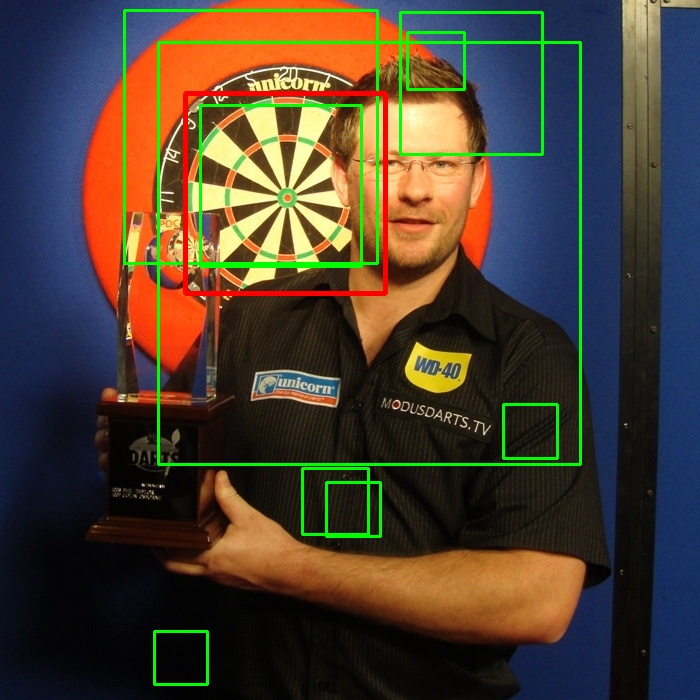
\includegraphics[width=\textwidth, height=20mm, keepaspectratio]{task2/out4.jpg}\label{fig:out4}}
  \hfill
  \subfloat[dart5.jpg]{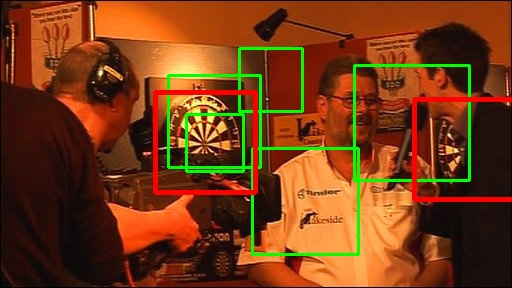
\includegraphics[width=\textwidth, height=20mm, keepaspectratio]{task2/out11.jpg}\label{fig:out11}}
   \hfill
  \subfloat[dart13.jpg]{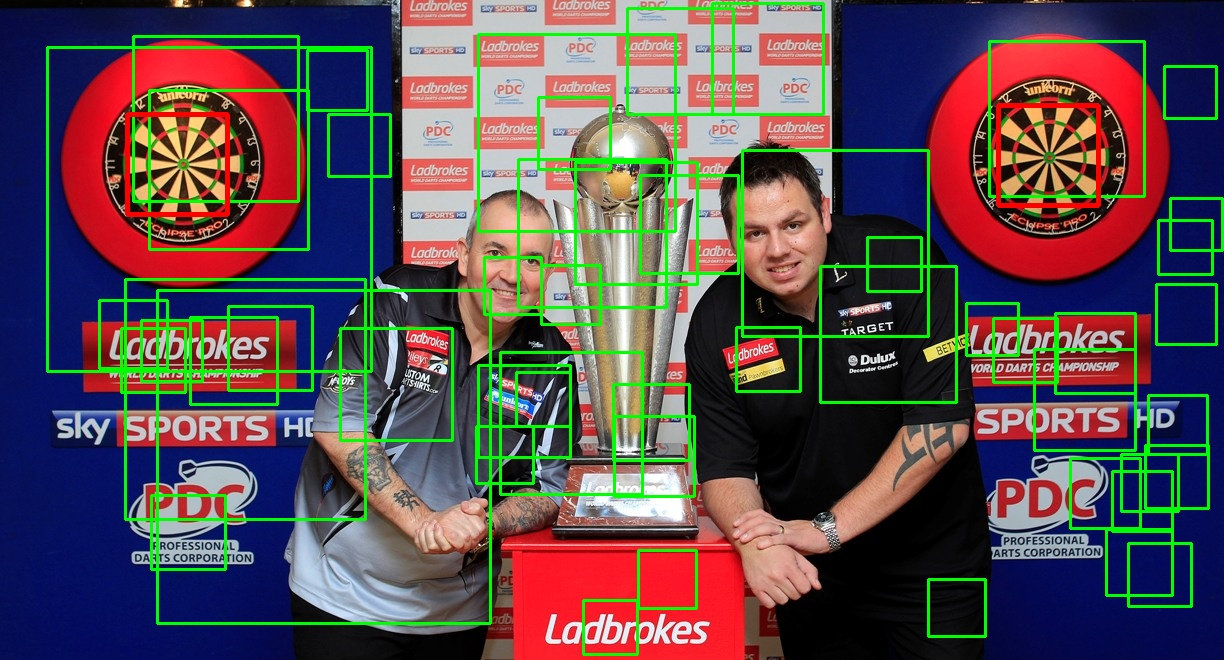
\includegraphics[width=\textwidth, height=20mm, keepaspectratio]{task2/out14.jpg}\label{fig:out14}}
   \hfill
  \subfloat[dart14.jpg]{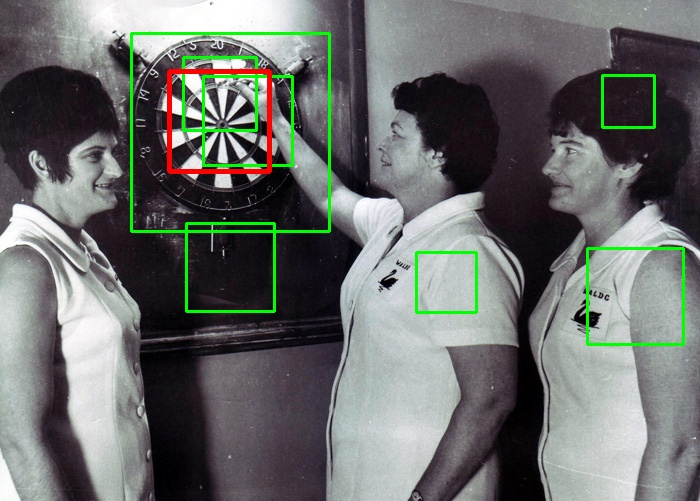
\includegraphics[width=\textwidth, height=20mm, keepaspectratio]{task2/out15.jpg}\label{fig:out15}}
   \hfill
   \caption{Result of the trained dartboard detector.}
\end{figure}

TODO: make this look beter?
The \(F_{1}\) of the images are:
\begin{multicols}{4}
    \begin{itemize}
		\item dart0.jpg - 0.14.
        \item dart1.jpg - 0.13.
        \item dart2.jpg - 0.12.
        \item dart3.jpg - 0.20.
        \item dart4.jpg - 0.20.
        \item dart5.jpg - 0.10.
        \item dart6.jpg - 0.17.
        \item dart7.jpg - 0.09.
        \item dart8.jpg - 0.13.
        \item dart9.jpg - 0.13.
        \item dart10.jpg - 0.11.
        \item dart11.jpg - 0.29.
        \item dart12.jpg - 0.33.
        \item dart13.jpg - 0.14.
        \item dart14.jpg - 0.07.
        \item dart15.jpg - 0.25.
    \end{itemize}
\end{multicols}

As the \(F_{1}\) score was calculated by the third rule and the TPR is 1, the
new equation becomes: \[\frac{2 \times hits}{detected + hits}\]. Also, the
\(F_{1}\) score is relatively low therefore there denominator is much bigger
and can conclude that the was a high number of detections. This means that
there were a lot of misses. The usefulness of the plot (Figure 2) is... I
dunno..

## Not sure we should use a new formula. We are using our own code to test if
there is a hit.

TODO: Talk about how it was shit but we can use the under fitting to out
advantage to combine with other classifier detectors.

\section{Integration with Shape Detectors}
\subsection*{Image Results}

\begin{figure}[H]
  \centering
  \subfloat[Threshold Gradient Magnitude.]{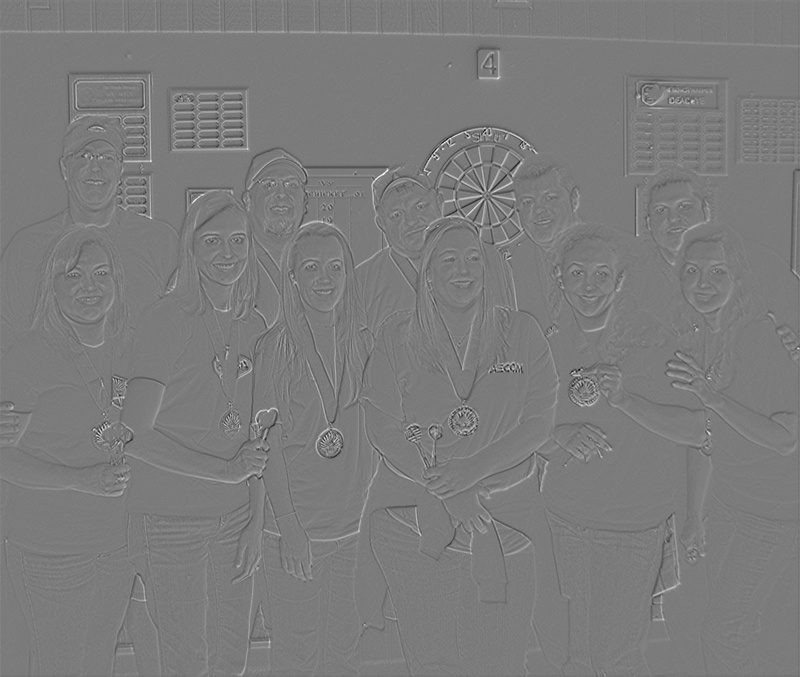
\includegraphics[width=\textwidth, height=20mm, keepaspectratio]{task3/mag5.jpg}\label{fig:mag1}}
  \hfill
  \subfloat[Hough Space]{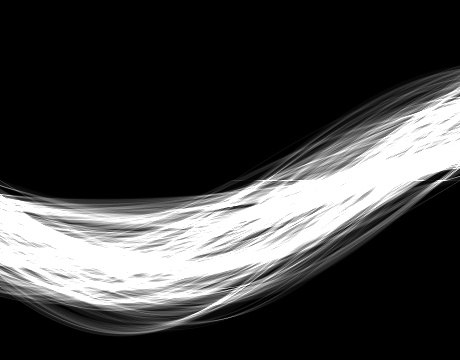
\includegraphics[width=\textwidth, height=20mm, keepaspectratio]{task3/hough5.jpg}\label{fig:hough1}}
   \hfill
  \subfloat[Result]{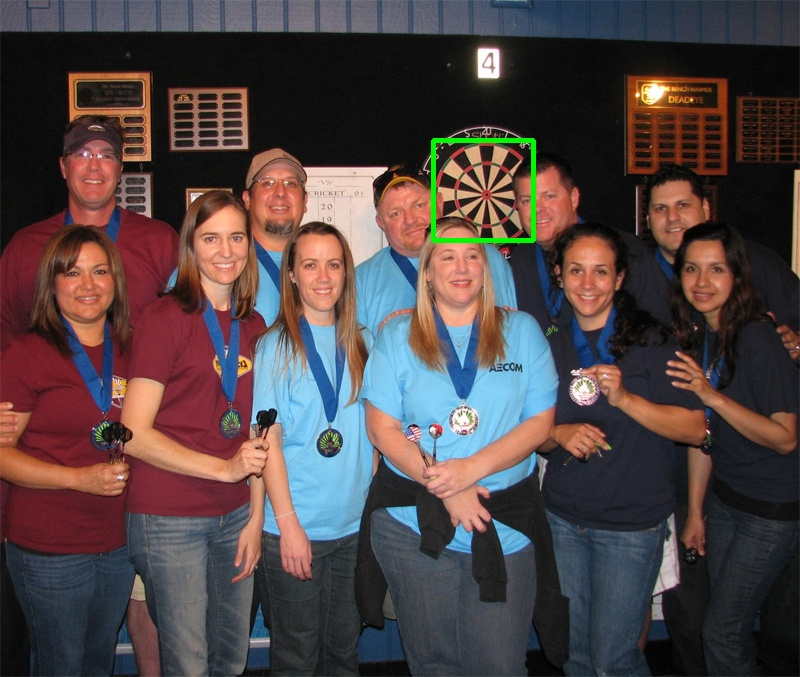
\includegraphics[width=\textwidth, height=20mm, keepaspectratio]{task3/out5.jpg}\label{fig:result1}}
   \hfill
   \caption{dart5.jpg shows the merits of the detector.}
\end{figure}

\begin{figure}[H]
  \centering
  \subfloat[Threshold Gradient Magnitude.]{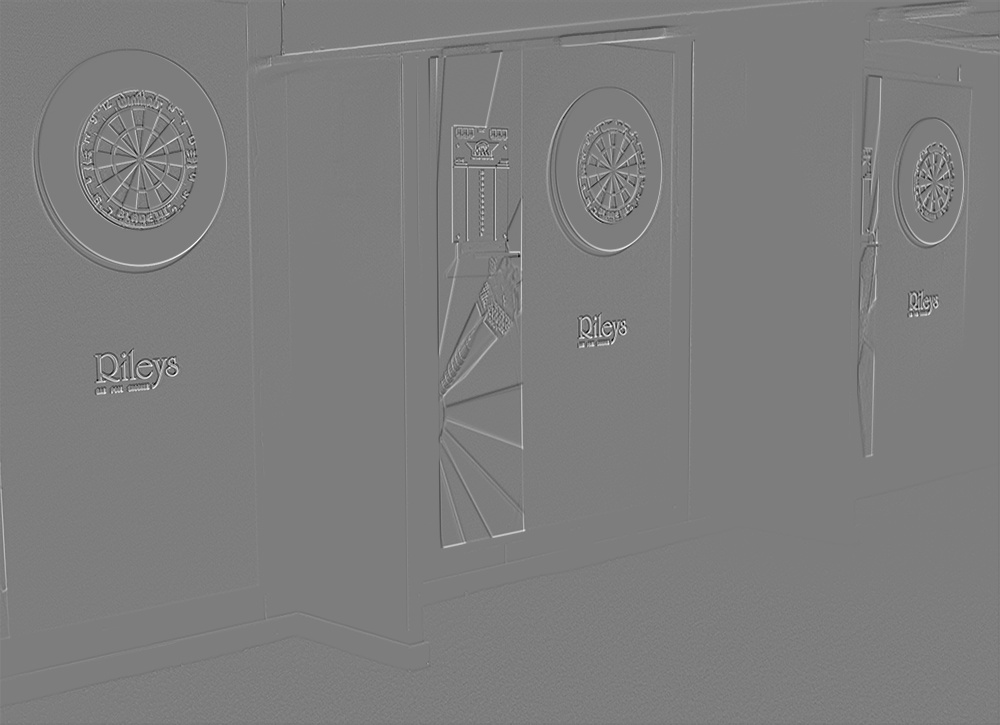
\includegraphics[width=\textwidth, height=20mm, keepaspectratio]{task3/mag10.jpg}\label{fig:mag2}}
  \hfill
  \subfloat[Hough Space]{
\includegraphics[width=\textwidth, height=20mm, keepaspectratio]{task3/hough10.jpg}\label{fig:hough2}}
   \hfill
  \subfloat[Result]{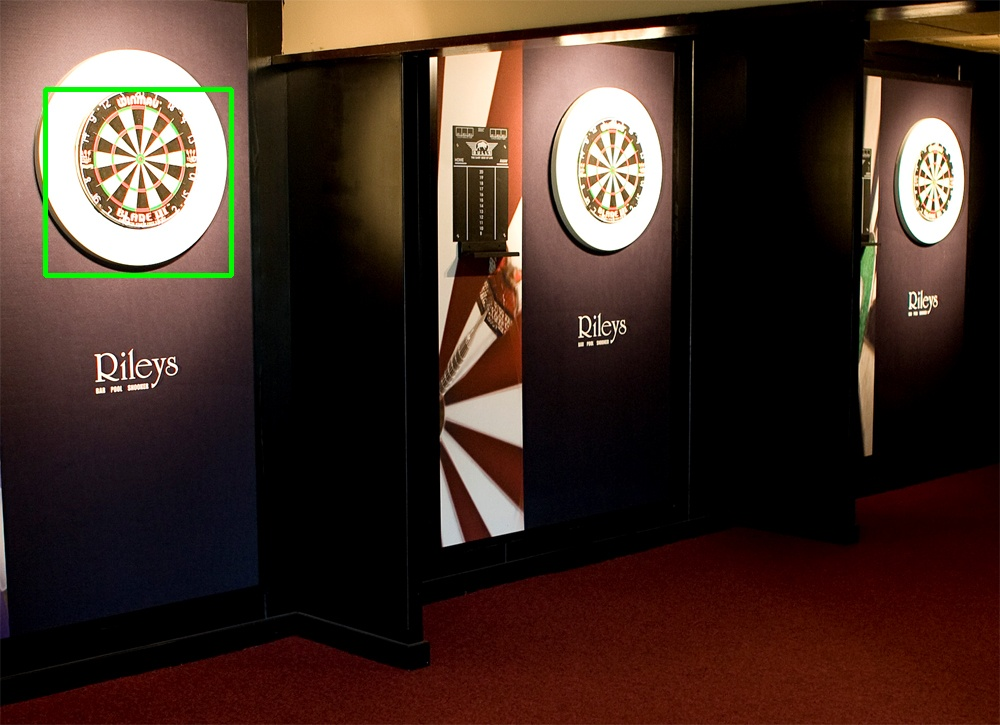
\includegraphics[width=\textwidth, height=20mm, keepaspectratio]{task3/out10.jpg}\label{fig:result2}}
   \hfill
   \caption{dart10.jpg shows the limitations of the detector.}
\end{figure}


\subsection*{Merits and Limitations}
Our new dartboard detector did considerably better than the previous, achieving
an overall \(F_{1}\) score ${0.767}$ with the previous being ${0.163 == check
this}$. This detector adds more classifiers when analysing images meaning that
the large set of detections with many negative hits, is able to be reduced by
combining each classifier result. This detector works optimally with images
where dartboards are in good lighting and are facing straight at the camera in
the scene. As shown in the dart10.jpg image, the detector failed to detect two
dartboards that are at an angle. This is because of the circle and line Hough
transformation being used, struggle to detect these.
TODO: Talk about how we get the line detections - intersections etc.

\subsection*{Combination of Detectors}
\begin{figure}[H]
  \centering
  \subfloat[Flowchart representing the detector.]{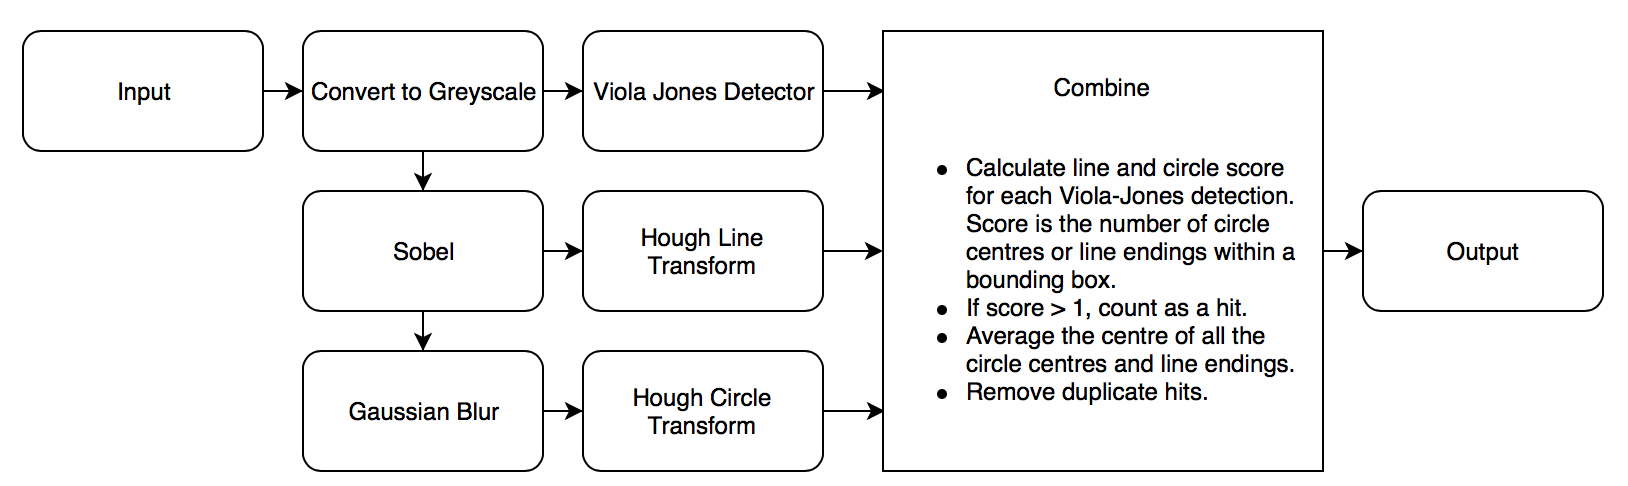
\includegraphics[width=\textwidth, height=40mm, keepaspectratio]{task3/flowchart.png}\label{fig:flowchart}}
\end{figure}

As shown, the Viola Jones detector results have a positive detection of every
dartboard in each image however have a large amount of false positives. Our
approach was to create new classifiers which would refine these hits down to
true positives by accepting Viola Jones hits that were also observed by our
line and circle detectors. This involves iterating through the set of Viola
hits, comparing whether any line or circle hits are contained in the Viola
bounding box, accepting if so, rejecting otherwise. If accepted, this hit would
change its location based on the average position of itself, along with its
combined detections. With the use of the circle detections, this also gave us
the ability to estimate the size of the dartboard also, taking the average
radius of included circles and including this in the approximation.  Once we
had achieved the new set of accepted detections we recognised that multiple
bounding boxes overlapped with one another. We thus combined all bounding boxes
that were overlapping, again averaging the coordinates and size, ensuring one
positive hit per dartboard.



\section{Improving the Detector}
\begin{itemize}
	\item ellipses
	\item find a better viola jones classifier
	\item adjust the parameters to fit better
	\item triangles
    \item make out3 brighter??
    \item otsu
\end{itemize}

\section{References}


\begin{table} [H]
\centering
\begin{tabular}{l| r | r | r | r | r | r}
Picture & Actual & Detected & Hit & Missed & \(F_{1}\) Score \\\hline
dart4 & 1 & 1 & 1 & 0 & 0 & 1\\
dart5 & 11 & 14 & 11 & 0 & 3 & 0.88 \\
dart13 & 1 & 2 & 1 & 0 & 1 & 0.67 \\
dart14 & 2 & 6 & 2 & 0 & 4 & 0.5 \\
dart15 & 3 & 4 & 2 & 1 & 2 & 0.57
\end{tabular}
\caption{\label{tab:F1}Comparing the \(F_{1}\) Score of different images.}
\end{table}

TODO: make this bullet points

In order to improve our dartboard classifier, we considered further shapes
which help to classify a dartboard being present.  As such, we identified two
shapes to consider - ellipses and triangles.  We realised that some dartboards
had been not been identified by our classifier due to not being detected by
circles with dartboards that are at an angle.  By using ellipse shapes we would
be able to capture this shape of valid dartboards.  We also chose to consider
triangle shapes inside images to detect dartboards.  This is because all
dartboards have distinct triangles contained that will give more detections
that can be combined in our detector.

Detecting both triangle and ellipse shapes is achieved by first applying the
Canny edge detector on the grey scale input image.  The Canny edge detector,
developed by  John F. Canny in 1986. [add citation] and works by calculating
the gradient magnitude of each pixel. To determine whether each pixel is part
of an edge two thresholds are applied, pixels higher than the larger threshold
are considered pixels on an edge, pixels below the lower threshold are
discarded and pixels in-between the two thresholds are considered edges only if
they are connected to a pixel that is above the higher threshold.  In order to
select an appropriate threshold for each image, the Otsu method can be applied.
[https://en.wikipedia.org/wiki/Otsu%27s_method]

The Otsu method is used to determine the largest threshold input for the Canny
edge detector.  TODO: Talk about how the method works.  The lower threshold
value is one third of the returning value from the Otsu method.

If a pixel gradient is higher than the upper threshold, the pixel is accepted
as an edge If a pixel gradient value is below the lower threshold, then it is
rejected.  If the pixel gradient is between the two thresholds, then it will be
accepted only if it is connected to a pixel that is above the upper threshold.
Canny recommended a upper:lower ratio between 2:1 and 3:1.

F1 score = .86666673333333333333

TODO: talk about surf
We use a scoring system with surf
We cluster surfs together togther that count as the same object

\end{document}
